\chapter{ĐẶC TẢ YÊU CẦU PHẦN MỀM (SRS)}

\section{Giới thiệu}

Tài liệu Đặc tả yêu cầu phần mềm (Software Requirements Specification - SRS) mô tả đầy đủ các yêu cầu của hệ thống Chatbot hỗ trợ học tập ứng dụng Retrieval-Augmented Generation (RAG) và Fine-Tuning. Tài liệu đóng vai trò là cơ sở để nhóm phát triển tiến hành thiết kế, triển khai, kiểm thử và đánh giá hệ thống.

Các yêu cầu được xây dựng dựa trên nhu cầu thực tế của sinh viên trong việc tra cứu tài liệu học tập, đồng thời hỗ trợ nghiên cứu và so sánh hiệu quả giữa hai phương pháp RAG và Fine-Tuning.

\section{Mục đích}

Mục đích của tài liệu SRS là:

\begin{itemize}
	\item Xác định đầy đủ các chức năng mà hệ thống cần cung cấp.
	\item Xác định các yêu cầu phi chức năng.
	\item Làm cơ sở cho việc thiết kế hệ thống.
	\item Hỗ trợ kiểm thử và nghiệm thu sản phẩm.
	\item Giảm sai lệch giữa yêu cầu và quá trình phát triển.
\end{itemize}

\section{Phạm vi hệ thống}

Hệ thống Chatbot được xây dựng nhằm hỗ trợ sinh viên đặt câu hỏi liên quan đến học tập và nhận câu trả lời từ mô hình AI.

Hệ thống cung cấp hai phương pháp xử lý:

\begin{itemize}
	\item Chatbot sử dụng Retrieval-Augmented Generation (RAG).
	\item Chatbot sử dụng mô hình Fine-Tuning.
\end{itemize}

Ngoài ra hệ thống còn cho phép quản trị viên quản lý tài liệu, theo dõi quá trình Fine-Tuning, đánh giá hiệu quả mô hình và xuất báo cáo thống kê.

\section{Các tác nhân của hệ thống}

Hệ thống gồm các tác nhân chính:

\begin{itemize}
	
	\item Sinh viên
	
	\item Quản trị viên
	
	\item Mô hình AI
	
	\item Kho tài liệu môn học
	
	\item Hệ thống Fine-Tuning
	
\end{itemize}

\section{Biểu đồ ngữ cảnh (Context Diagram)}

Biểu đồ Context mô tả hệ thống ở mức tổng quát nhất, thể hiện các tác nhân bên ngoài và luồng dữ liệu trao đổi với hệ thống.

\begin{figure}[H]
	\centering
	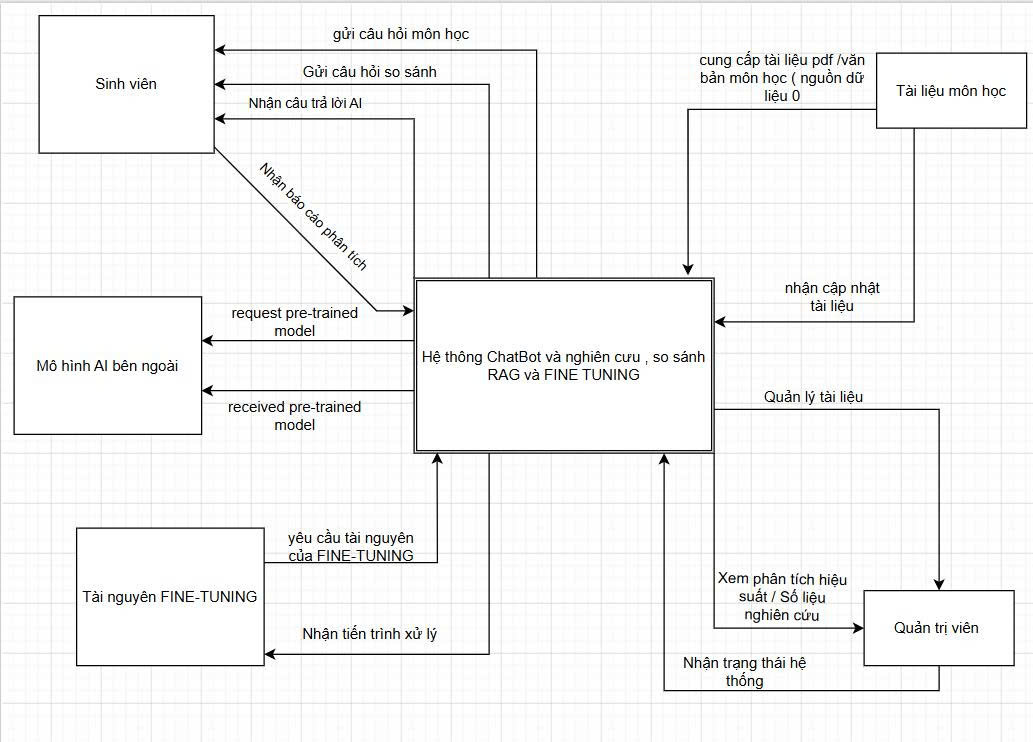
\includegraphics[width=\textwidth]{images/context.png}
	\caption{Biểu đồ Context của hệ thống}
	\label{fig:context}
\end{figure}

Trong biểu đồ Context, hệ thống Chatbot đóng vai trò trung tâm tiếp nhận và xử lý mọi yêu cầu từ các tác nhân bên ngoài.

Sinh viên gửi câu hỏi về môn học hoặc yêu cầu so sánh giữa hai phương pháp RAG và Fine-Tuning. Sau khi xử lý, hệ thống trả về câu trả lời cùng các báo cáo phân tích nếu người dùng yêu cầu.

Kho tài liệu môn học cung cấp dữ liệu PDF, Word và các tài liệu học tập để phục vụ quá trình truy xuất thông tin của RAG.

Mô hình AI bên ngoài được sử dụng để sinh câu trả lời thông minh dựa trên Prompt do hệ thống tạo ra.

Tài nguyên Fine-Tuning chịu trách nhiệm cung cấp môi trường huấn luyện và cập nhật mô hình mới.

Quản trị viên có quyền quản lý tài liệu, theo dõi trạng thái hệ thống, xem thống kê và đánh giá hiệu quả của các mô hình AI.

\section{Biểu đồ Use Case}

Biểu đồ Use Case mô tả toàn bộ các chức năng mà hệ thống cung cấp cho từng tác nhân.

\begin{figure}[H]
	\centering
	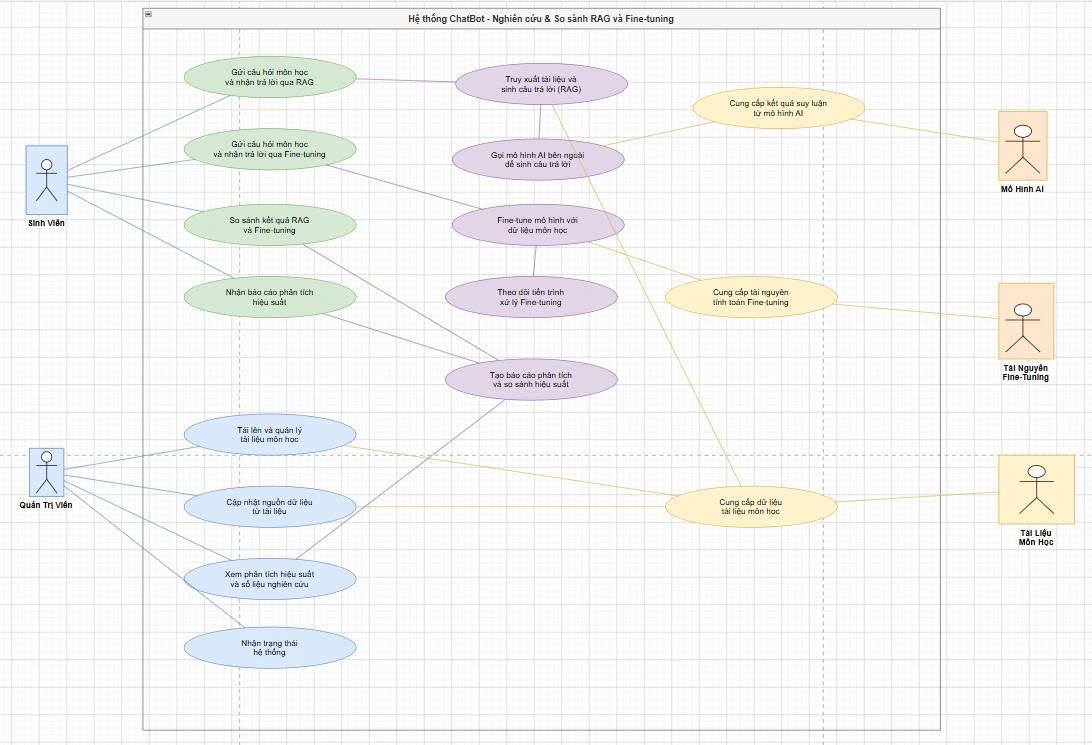
\includegraphics[width=\textwidth]{images/usecase.png}
	\caption{Biểu đồ Use Case}
	\label{fig:usecase}
\end{figure}

Biểu đồ Use Case cho thấy hệ thống gồm hai nhóm người dùng chính là Sinh viên và Quản trị viên.

Sinh viên có thể:

\begin{itemize}
	
	\item Gửi câu hỏi bằng RAG.
	
	\item Gửi câu hỏi bằng Fine-Tuning.
	
	\item So sánh kết quả giữa hai phương pháp.
	
	\item Xem báo cáo đánh giá.
	
\end{itemize}

Quản trị viên có thể:

\begin{itemize}
	
	\item Tải lên tài liệu mới.
	
	\item Quản lý kho dữ liệu.
	
	\item Cập nhật tài liệu.
	
	\item Theo dõi trạng thái hệ thống.
	
	\item Xem báo cáo phân tích.
	
	\item Quản lý quá trình Fine-Tuning.
	
\end{itemize}

Trong quá trình xử lý, hệ thống sẽ gọi tới mô hình AI, truy xuất dữ liệu từ ChromaDB theo cơ chế RAG hoặc sử dụng mô hình Fine-Tuning để sinh câu trả lời.

\section{Yêu cầu chức năng}

Hệ thống cần đáp ứng các yêu cầu chức năng sau:

\begin{enumerate}
	
	\item Cho phép sinh viên nhập câu hỏi.
	
	\item Truy xuất dữ liệu từ ChromaDB.
	
	\item Sinh câu trả lời bằng RAG.
	
	\item Sinh câu trả lời bằng Fine-Tuning.
	
	\item So sánh kết quả giữa hai phương pháp.
	
	\item Lưu lịch sử hội thoại.
	
	\item Quản lý tài liệu học tập.
	
	\item Quản lý người dùng.
	
	\item Sinh báo cáo thống kê.
	
	\item Theo dõi tiến trình Fine-Tuning.
	
\end{enumerate}

\section{Yêu cầu phi chức năng}

\begin{enumerate}
	
	\item\textbf{\large Hiệu năng}: Thời gian phản hồi trung bình nhỏ hơn 5 giây đối với câu hỏi thông thường. 
	
	\item\textbf{\large Độ chính xác}: Hệ thống ưu tiên trả lời dựa trên tài liệu môn học trước khi sử dụng tri thức tổng quát của mô hình AI.
	
	\item\textbf{\large Khả năng mở rộng}: Có thể bổ sung tài liệu mới mà không cần thay đổi chương trình.
	
	\item\textbf{\large Bảo mật}: Chỉ quản trị viên mới được phép cập nhật tài liệu và quản lý hệ thống.
	
	\item\textbf{\large Khả dụng} : Hệ thống hoạt động liên tục và hỗ trợ nhiều người dùng đồng thời thông qua FastAPI.
	
	
\end{enumerate}

\section{Kết luận chương}

Chương này đã trình bày đầy đủ đặc tả yêu cầu phần mềm của hệ thống Chatbot hỗ trợ học tập, bao gồm mục đích, phạm vi, các yêu cầu chức năng, yêu cầu phi chức năng cùng hai sơ đồ quan trọng là Context Diagram và Use Case Diagram. Đây là cơ sở để tiến hành thiết kế kiến trúc và triển khai hệ thống trong các chương tiếp theo.